\documentclass{article}
\usepackage{graphicx}

\usepackage{titling}
\newcommand{\subtitle}[1]{%
  \posttitle{%
    \par\end{center}
    \begin{center}\large#1\end{center}
    \vskip0.5em}%
}

\begin{document}

\title{Software Entwicklung Projekt - Sonjas Coursera}
\subtitle{Allgemeine Informatik - IN7 - Prof. Dr. Jobst}
\author{Sonja Riethig}

\maketitle

\begin{abstract}
Das Projekt "Sonjas Coursera" implementiert einen einfachen Online-Kurs - Anbieter. Im Folgenden werden die Anforderungen an das Projekt mithilfe von Diagrammen mit Anmerkungen dargestellt.
\end{abstract}

\section{Klassendiagramm}

\begin{figure}
    \centering
    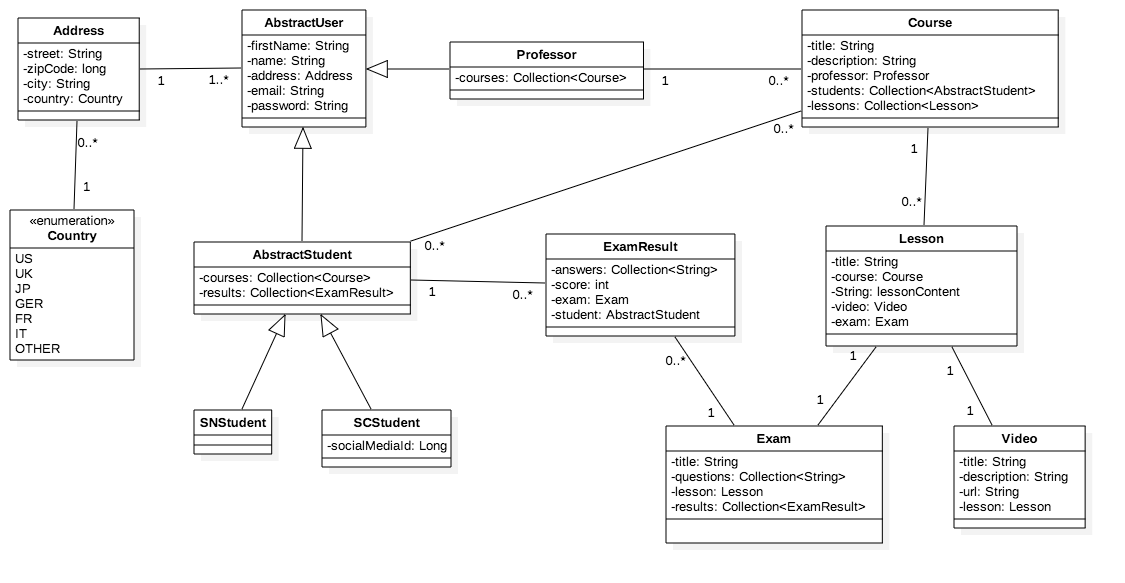
\includegraphics[width=15cm]{./UML/classDiagram.png}
    \caption{Klassendiagramm}
    \label{Klassendiagramm}
\end{figure}

\section{Use Cases}

\subsection{SCStudent - mit Emailadresse anmelden}
\subsection{AbstractStudent - Kurs buchen}
\subsection{SNStudent - �ber Sebastians Nutwork registrieren und anmelden}

\section{Komponentendiagramm}

\begin{equation}
    \label{simple_equation}
    \alpha = \sqrt{ \beta }
\end{equation}

\subsection{Subsection Heading Here}
Write your subsection text here.

\begin{figure}
    \centering
    %\includegraphics[width=3.0in]{myfigure}
    \caption{Simulation Results}
    \label{simulationfigure}
\end{figure}

\section{Conclusion}
Write your conclusion here.

\end{document}